\documentclass[11pt,a4paper]{article}
\usepackage[T2A]{fontenc}
\usepackage[utf8]{inputenc}
\usepackage[english,russian]{babel}
\usepackage{geometry,graphicx,amsmath,booktabs,longtable,float}
\geometry{margin=1.8cm}
\title{Сравнение модели Хилла--Клохесси--Уилтшира и кеплерова движения}
\author{Задание 1}
\date{}
\begin{document}

    \maketitle
    \section{Постановка и метод}
    Самостоятельно выбрана круговая опорная орбита радиуса $a=7000$ км, $\mu=398600.4418$
    км$^3$/с$^2$; $n=\sqrt{\mu/a^3}$. Относительные координаты заданы в системе RTN: $x$ радиально,
    $y$ вдоль движения, $z$ по нормали. Расчёт выполняется на двух периодах опорной орбиты, с 721
    моментом включая границы. Исследуются все $3\cdot3\cdot2\cdot5=90$ наборов.

    Для ХКУ использовано аналитическое решение системы $\ddot x-2n\dot y-3n^2x=0$, $\ddot y+2n\dot
    x=0$, $\ddot z+n^2z=0$. Во втором способе оба аппарата независимо рассчитываются численным
    интегрированием точных двухтельных уравнений $\ddot{\mathbf r}=-\mu\mathbf r/|\mathbf r|^3$ при
    допусках $10^{-10}$. Начальные состояния согласованы через $\mathbf r_2=\mathbf r_1+\rho$ и
    $\mathbf v_2=\mathbf v_1+\dot\rho+\boldsymbol\omega\times\rho$. На каждом шаге разность
    инерциальных положений проектируется в текущую вращающуюся систему опорного аппарата. Этим
    обеспечивается сравнение в одной системе и с одинаковыми начальными данными. Модель не учитывает
    возмущения и манёвры.

    Согласованные скорости заданы формулами $v_{x0}=ny_0/2$, $v_{y0}=-2nx_0$, $v_{z0}=0$. Для
    несогласованного варианта рассмотрены все четыре пары из $v_{x0},v_{y0}\in\{0,100\}$ м/с. Ошибка
    $\Delta(t)$ — евклидова норма разности относительных положений двух способов; таблица содержит
    её максимум и конечное значение, а также максимум расстояния между аппаратами по двухтельной
    модели, делённый на $a$.

    Согласованная скорость подбирается по начальному положению: условие $v_{y0}=-2nx_0$ устраняет
    вековой дрейф в модели ХКУ. Несогласованная скорость задаётся независимо от положения и может
    привести к постепенному расхождению аппаратов. Ограниченность при согласованной скорости
    относится к линейной модели ХКУ.

    \section{Анализ}
    При $x_0=0.1$ км согласованные скорости дают максимальные ошибки от $0.000016$ до $0.003205$ км
    по всем значениям $y_0,z_0$. При $x_0=10$ км этот диапазон составляет 0.265--0.269 км, а при
    $x_0=100$ км — 25.99--26.01 км. На этой сетке увеличение радиального смещения существенно
    усиливает нелинейные эффекты даже при согласованной скорости.

    При $x_0=0.1$ км и нулевых несогласованных скоростях максимум ошибки составляет 0.004--0.007 км;
    при $v_y=100$ м/с и $v_x=0$ — около 928 км, а при $v_x=100$ м/с и $v_y=0$ — 23--23.5 км.
    Следовательно, на выбранном интервале продольная скорость особенно сильно влияет на дрейф и
    ошибку. В наиболее расходящемся случае №65 ($x_0=100$ км, $y_0=z_0=0$, обе скорости по 100 м/с)
    максимум ошибки достигает 8978 км, а относительное расстояние — 11071 км. Отношение
    $\rho/a=1.58$ показывает явный выход за предпосылку малого относительного расстояния; прогноз
    ХКУ здесь следует рассматривать только как иллюстрацию отказа приближения.

    В таблице влияния $y_0$ и $z_0$ видны через сравнение строк с одинаковыми $x_0$ и скоростным
    вариантом; на выбранных диапазонах оно меньше, чем эффект 100 км радиального смещения или 100
    м/с продольной скорости. Конечность результатов на двух витках не гарантирует точности на более
    длинном интервале. Допуски численного интегрирования не являются оценкой погрешности самой
    модели ХКУ.

    \section{Примеры}
    Синим показан двухтельный расчёт, красным — ХКУ. В каждом PDF оси подбираются по данным;
    масштабы графиков разных случаев отличаются. Все 90 PDF находятся в \texttt{results/}, их номера
    совпадают с таблицей.
    \begin{figure}[H]
        \centering
        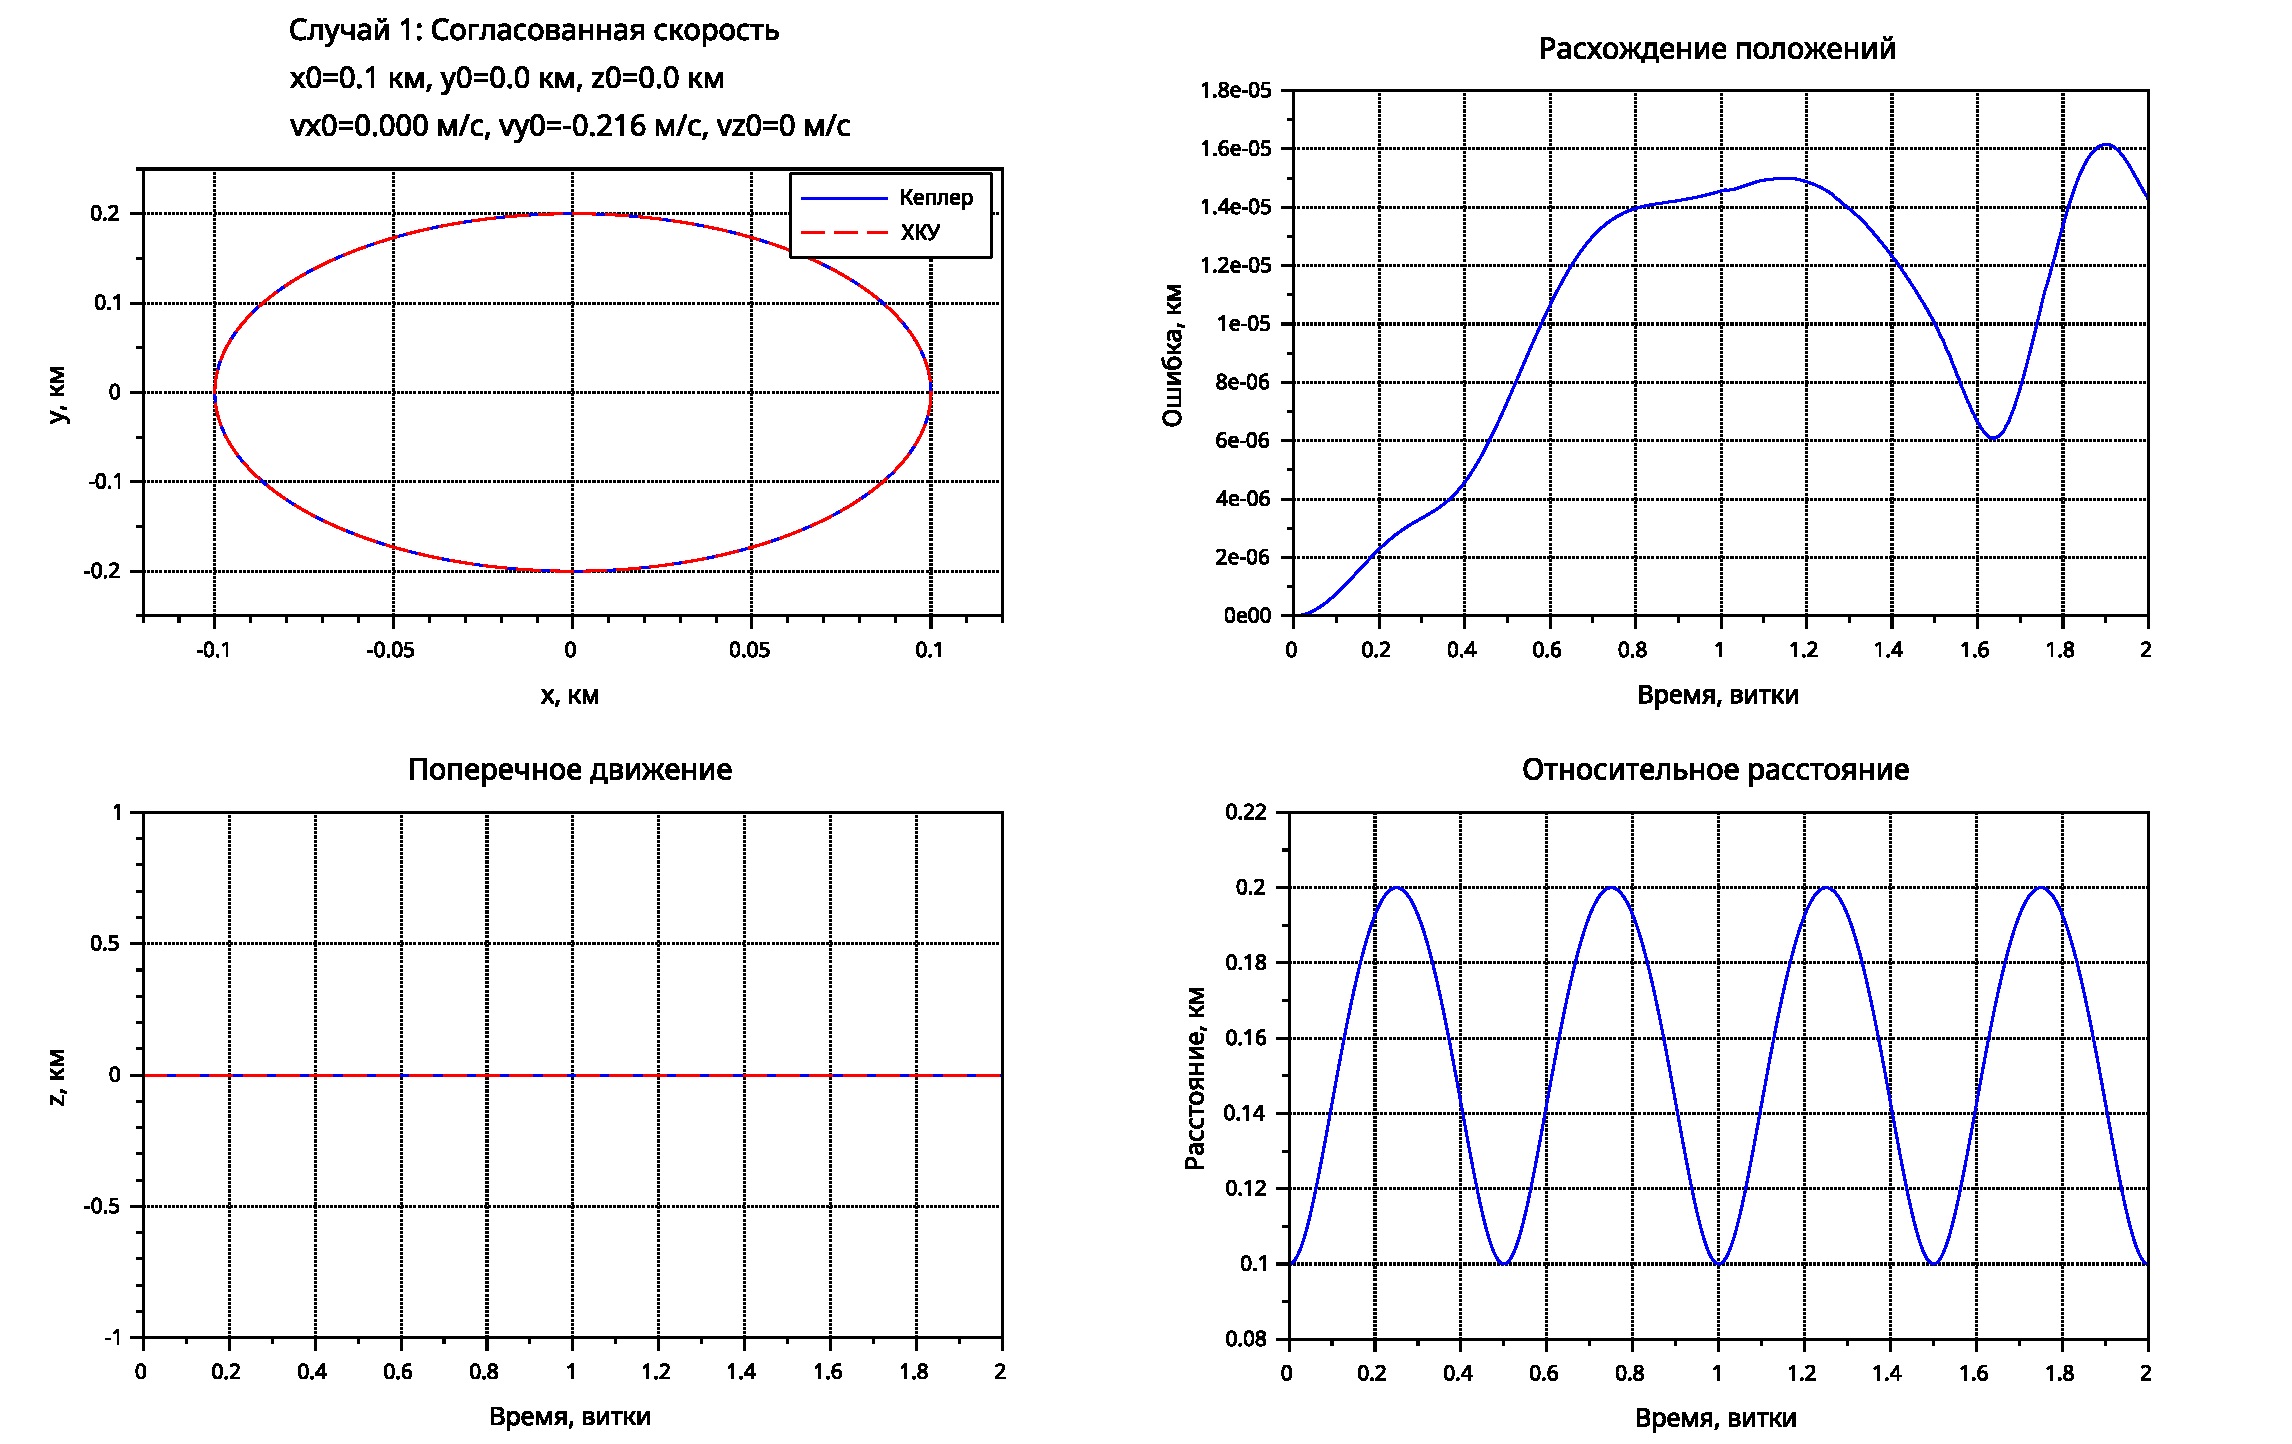
\includegraphics[width=.9\textwidth]{results/case_01.pdf}
        \caption{№1: малое смещение, согласованная скорость.}
    \end{figure}
    \begin{figure}[H]
        \centering
        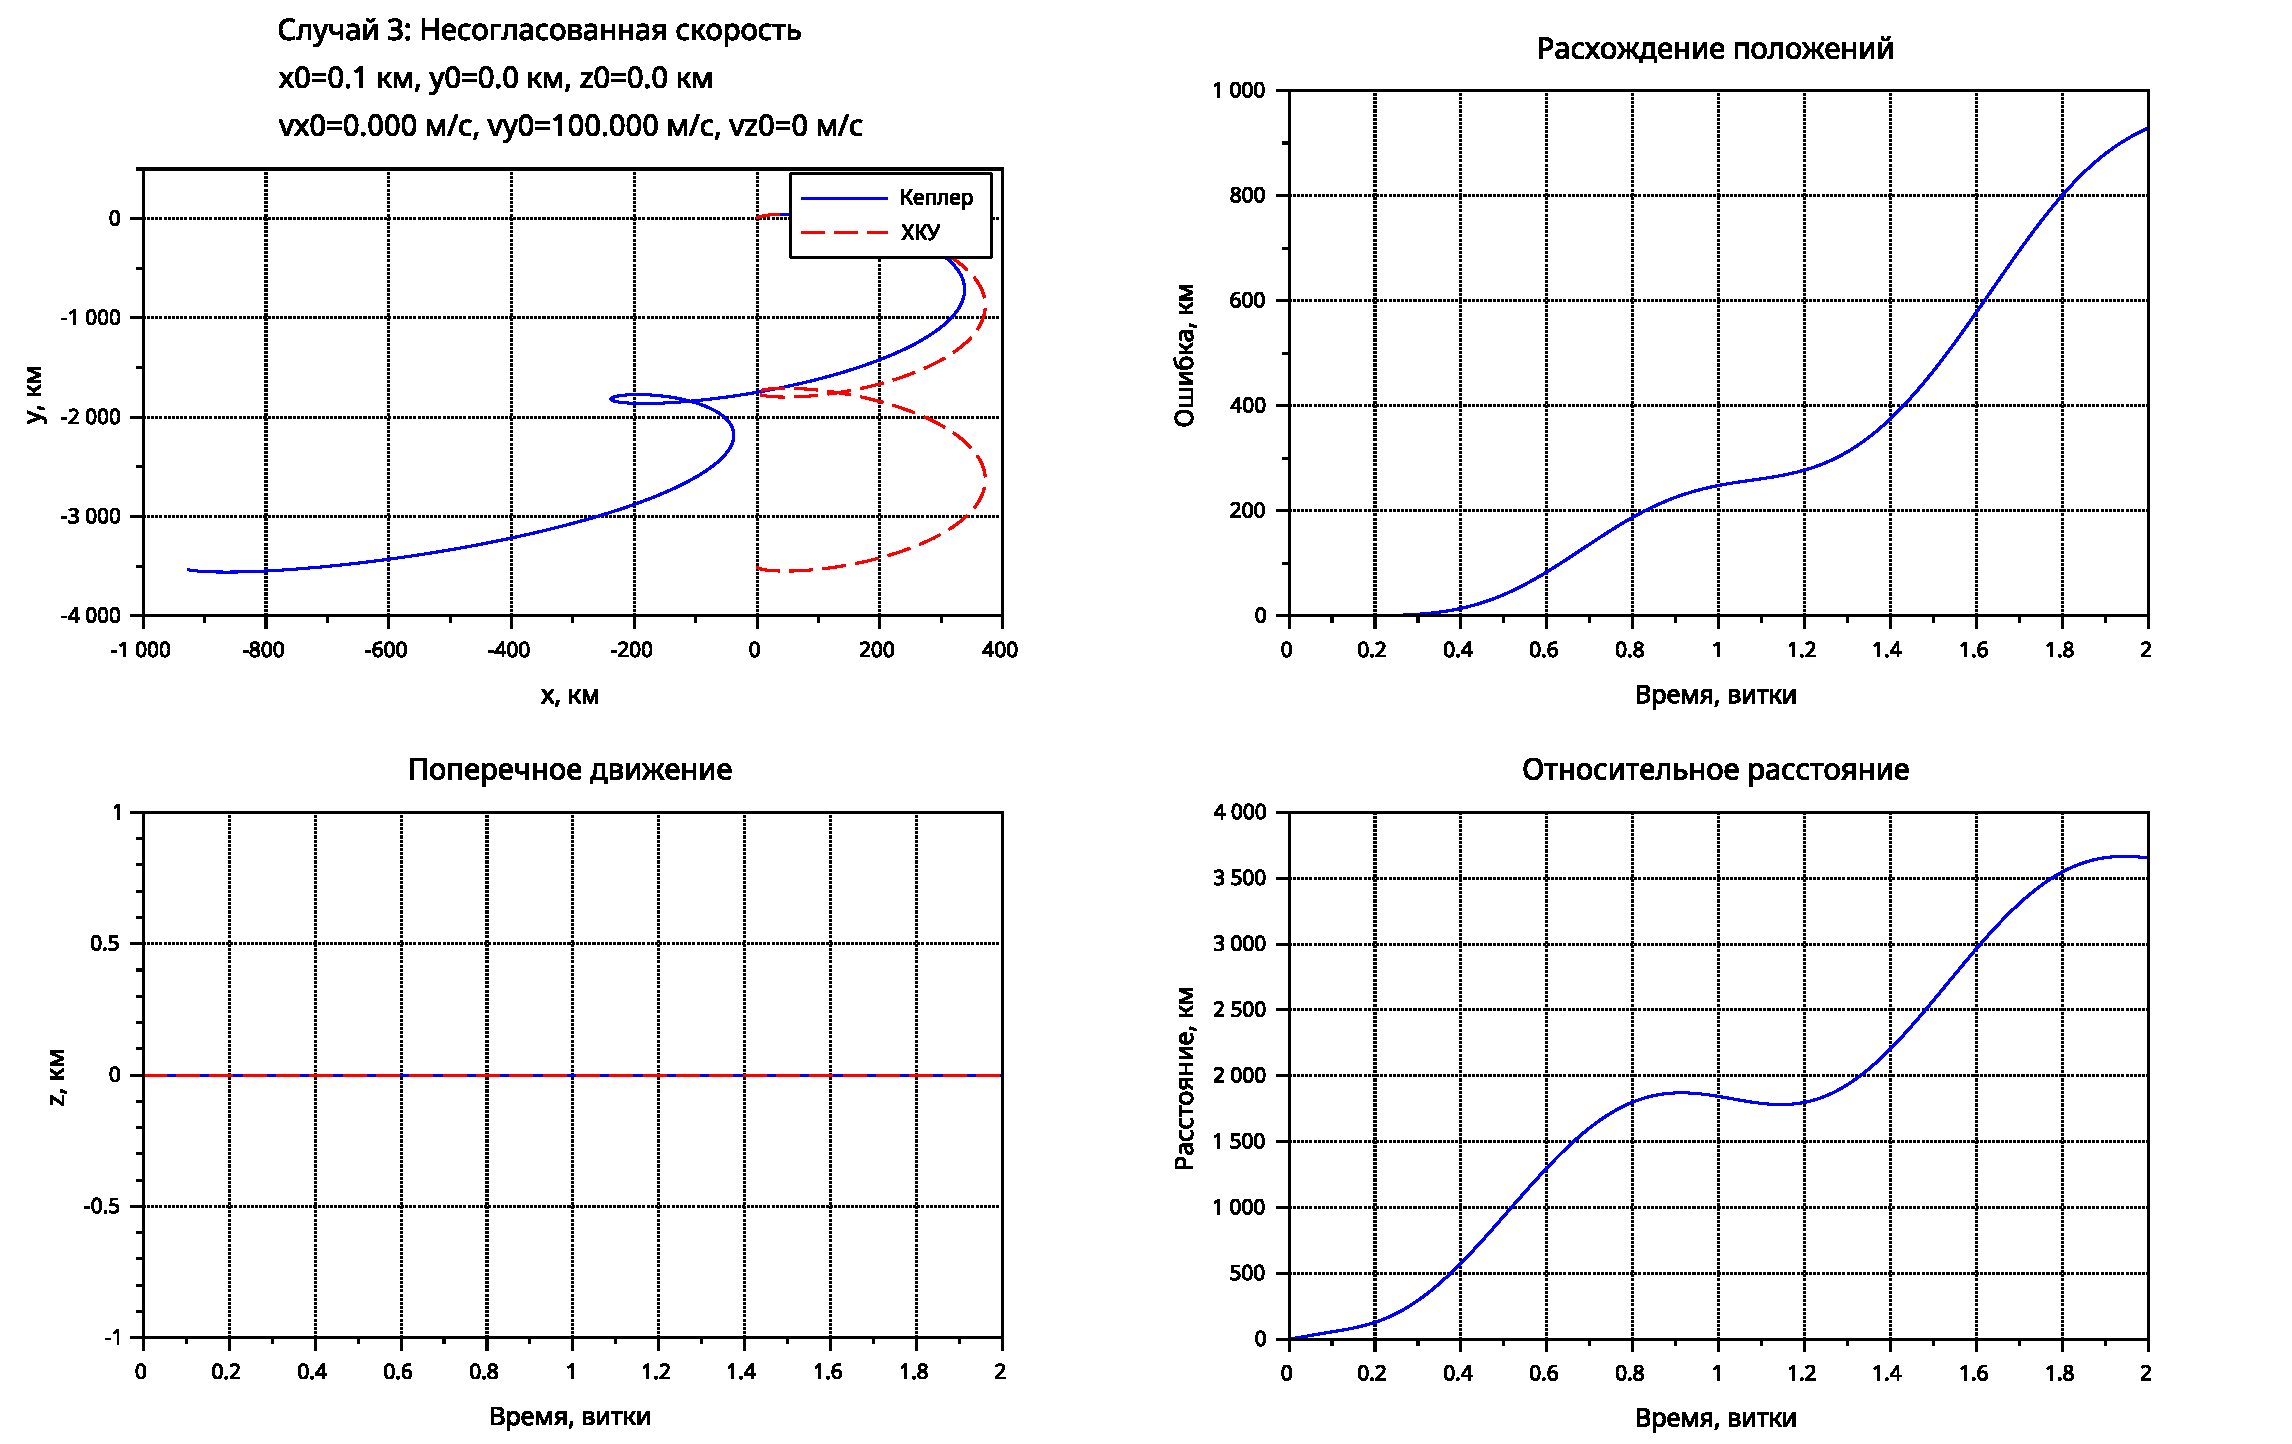
\includegraphics[width=.9\textwidth]{results/case_03.pdf}
        \caption{№3: малое смещение, несогласованная продольная скорость 100 м/с.}
    \end{figure}
    \begin{figure}[H]
        \centering
        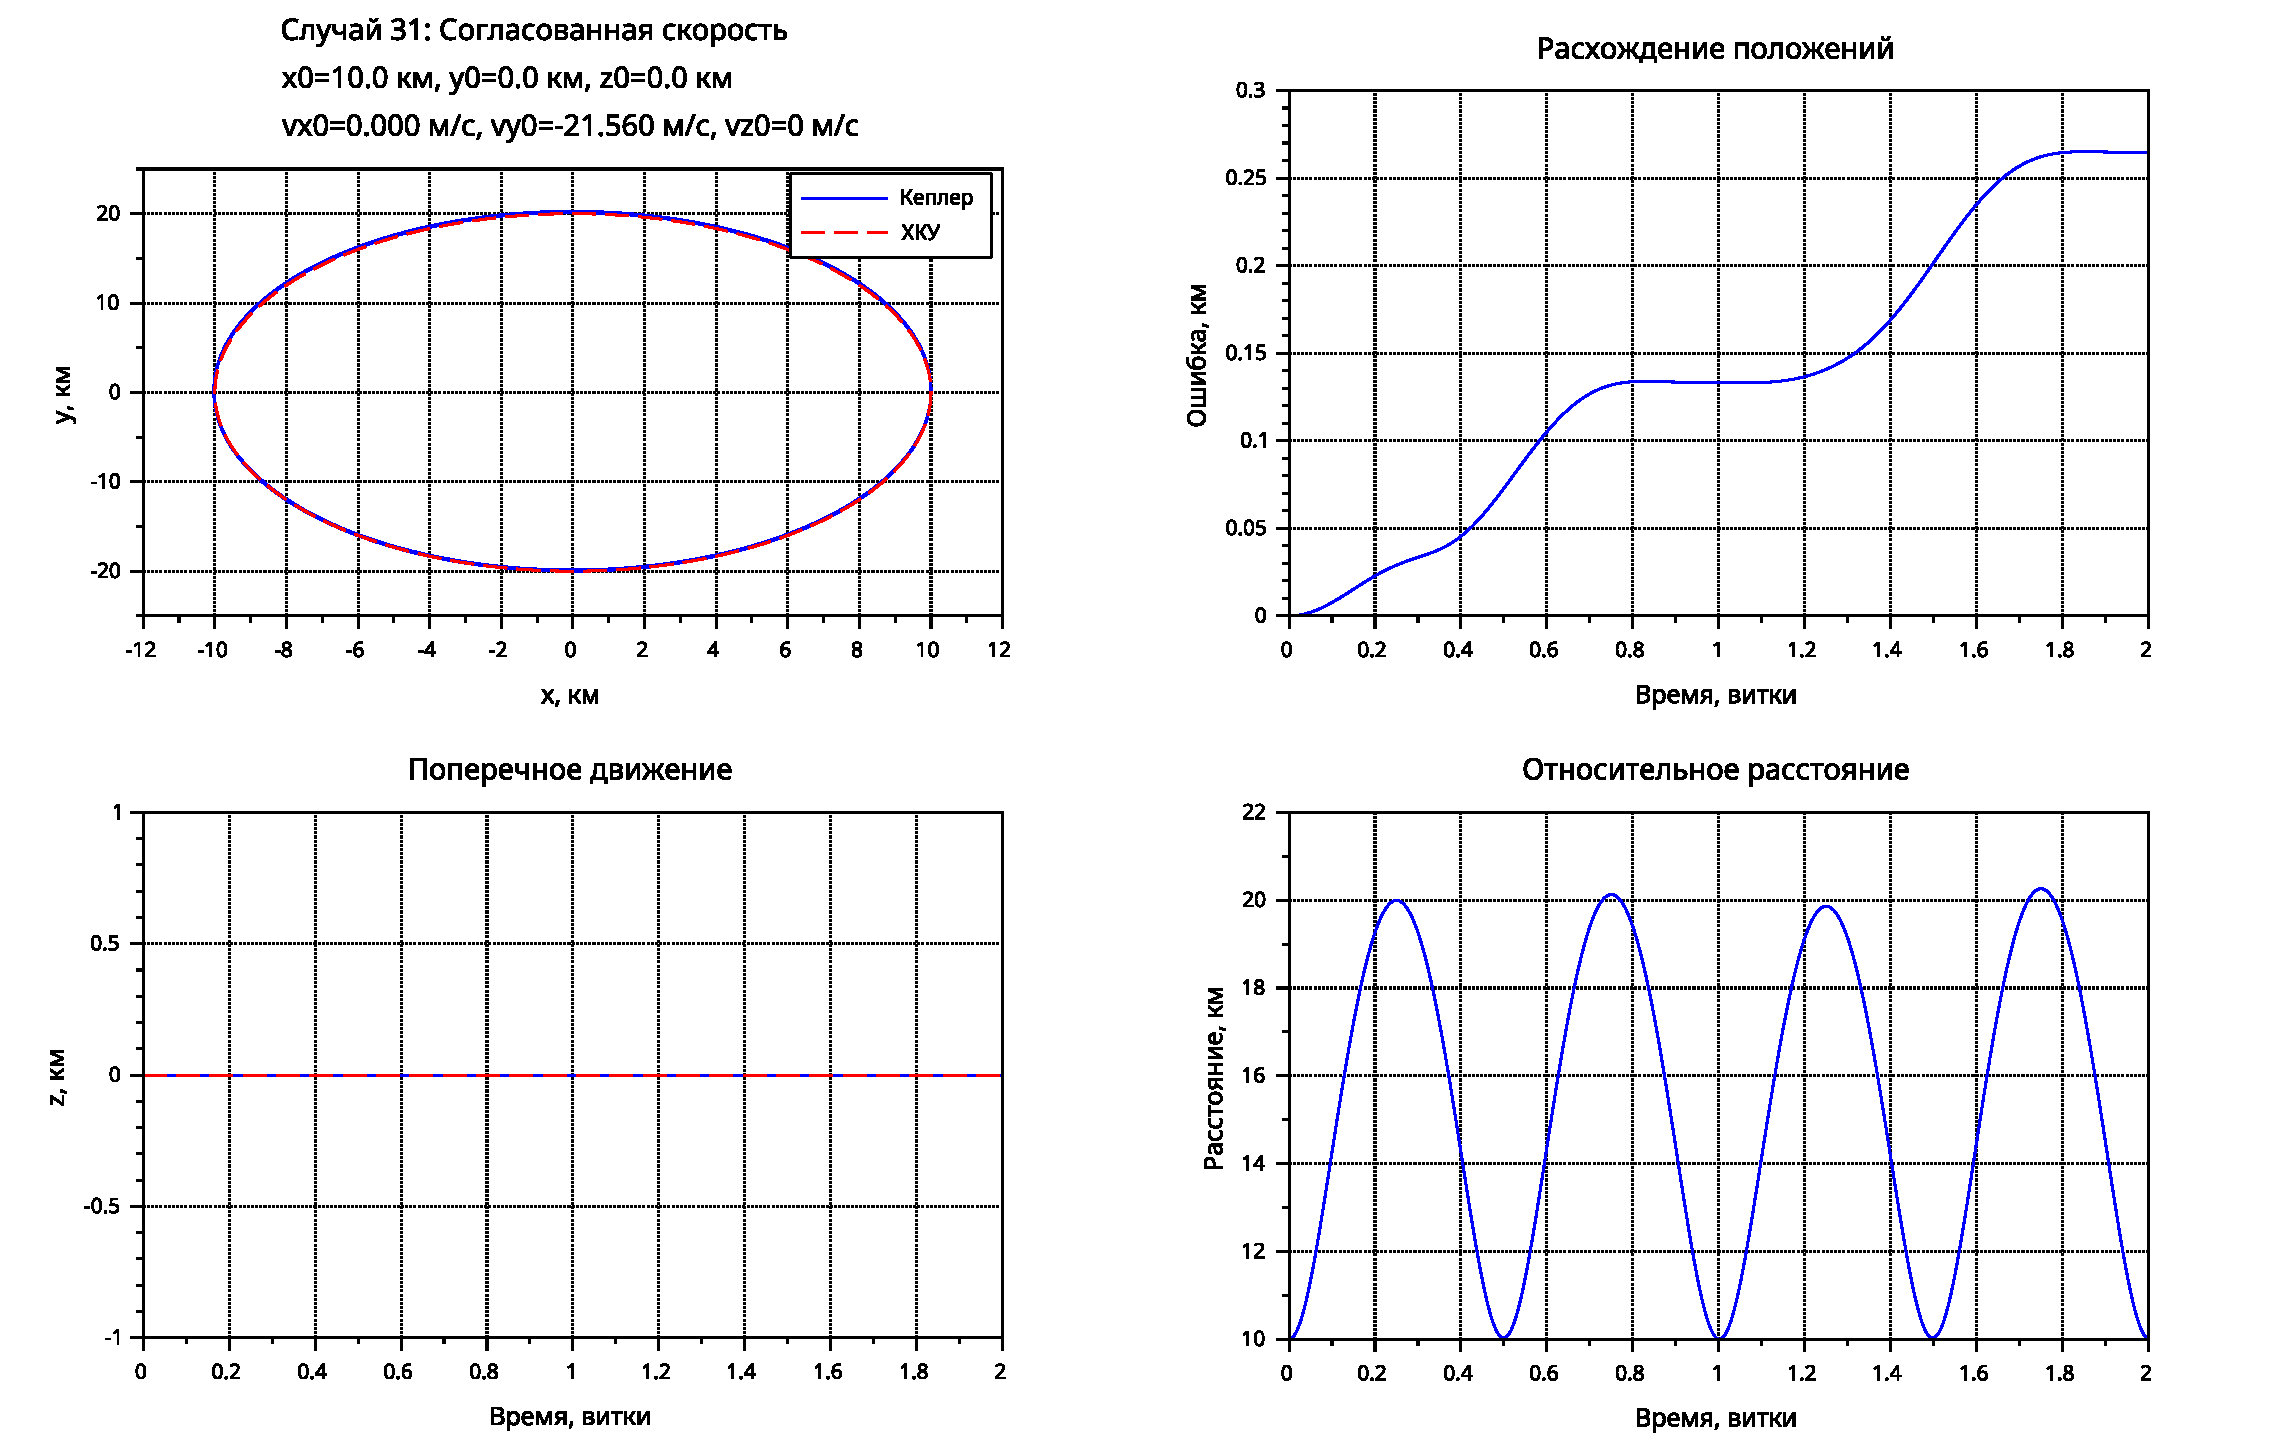
\includegraphics[width=.9\textwidth]{results/case_31.pdf}
        \caption{№31: радиальное смещение 10 км, согласованная скорость.}
    \end{figure}
    \begin{figure}[H]
        \centering
        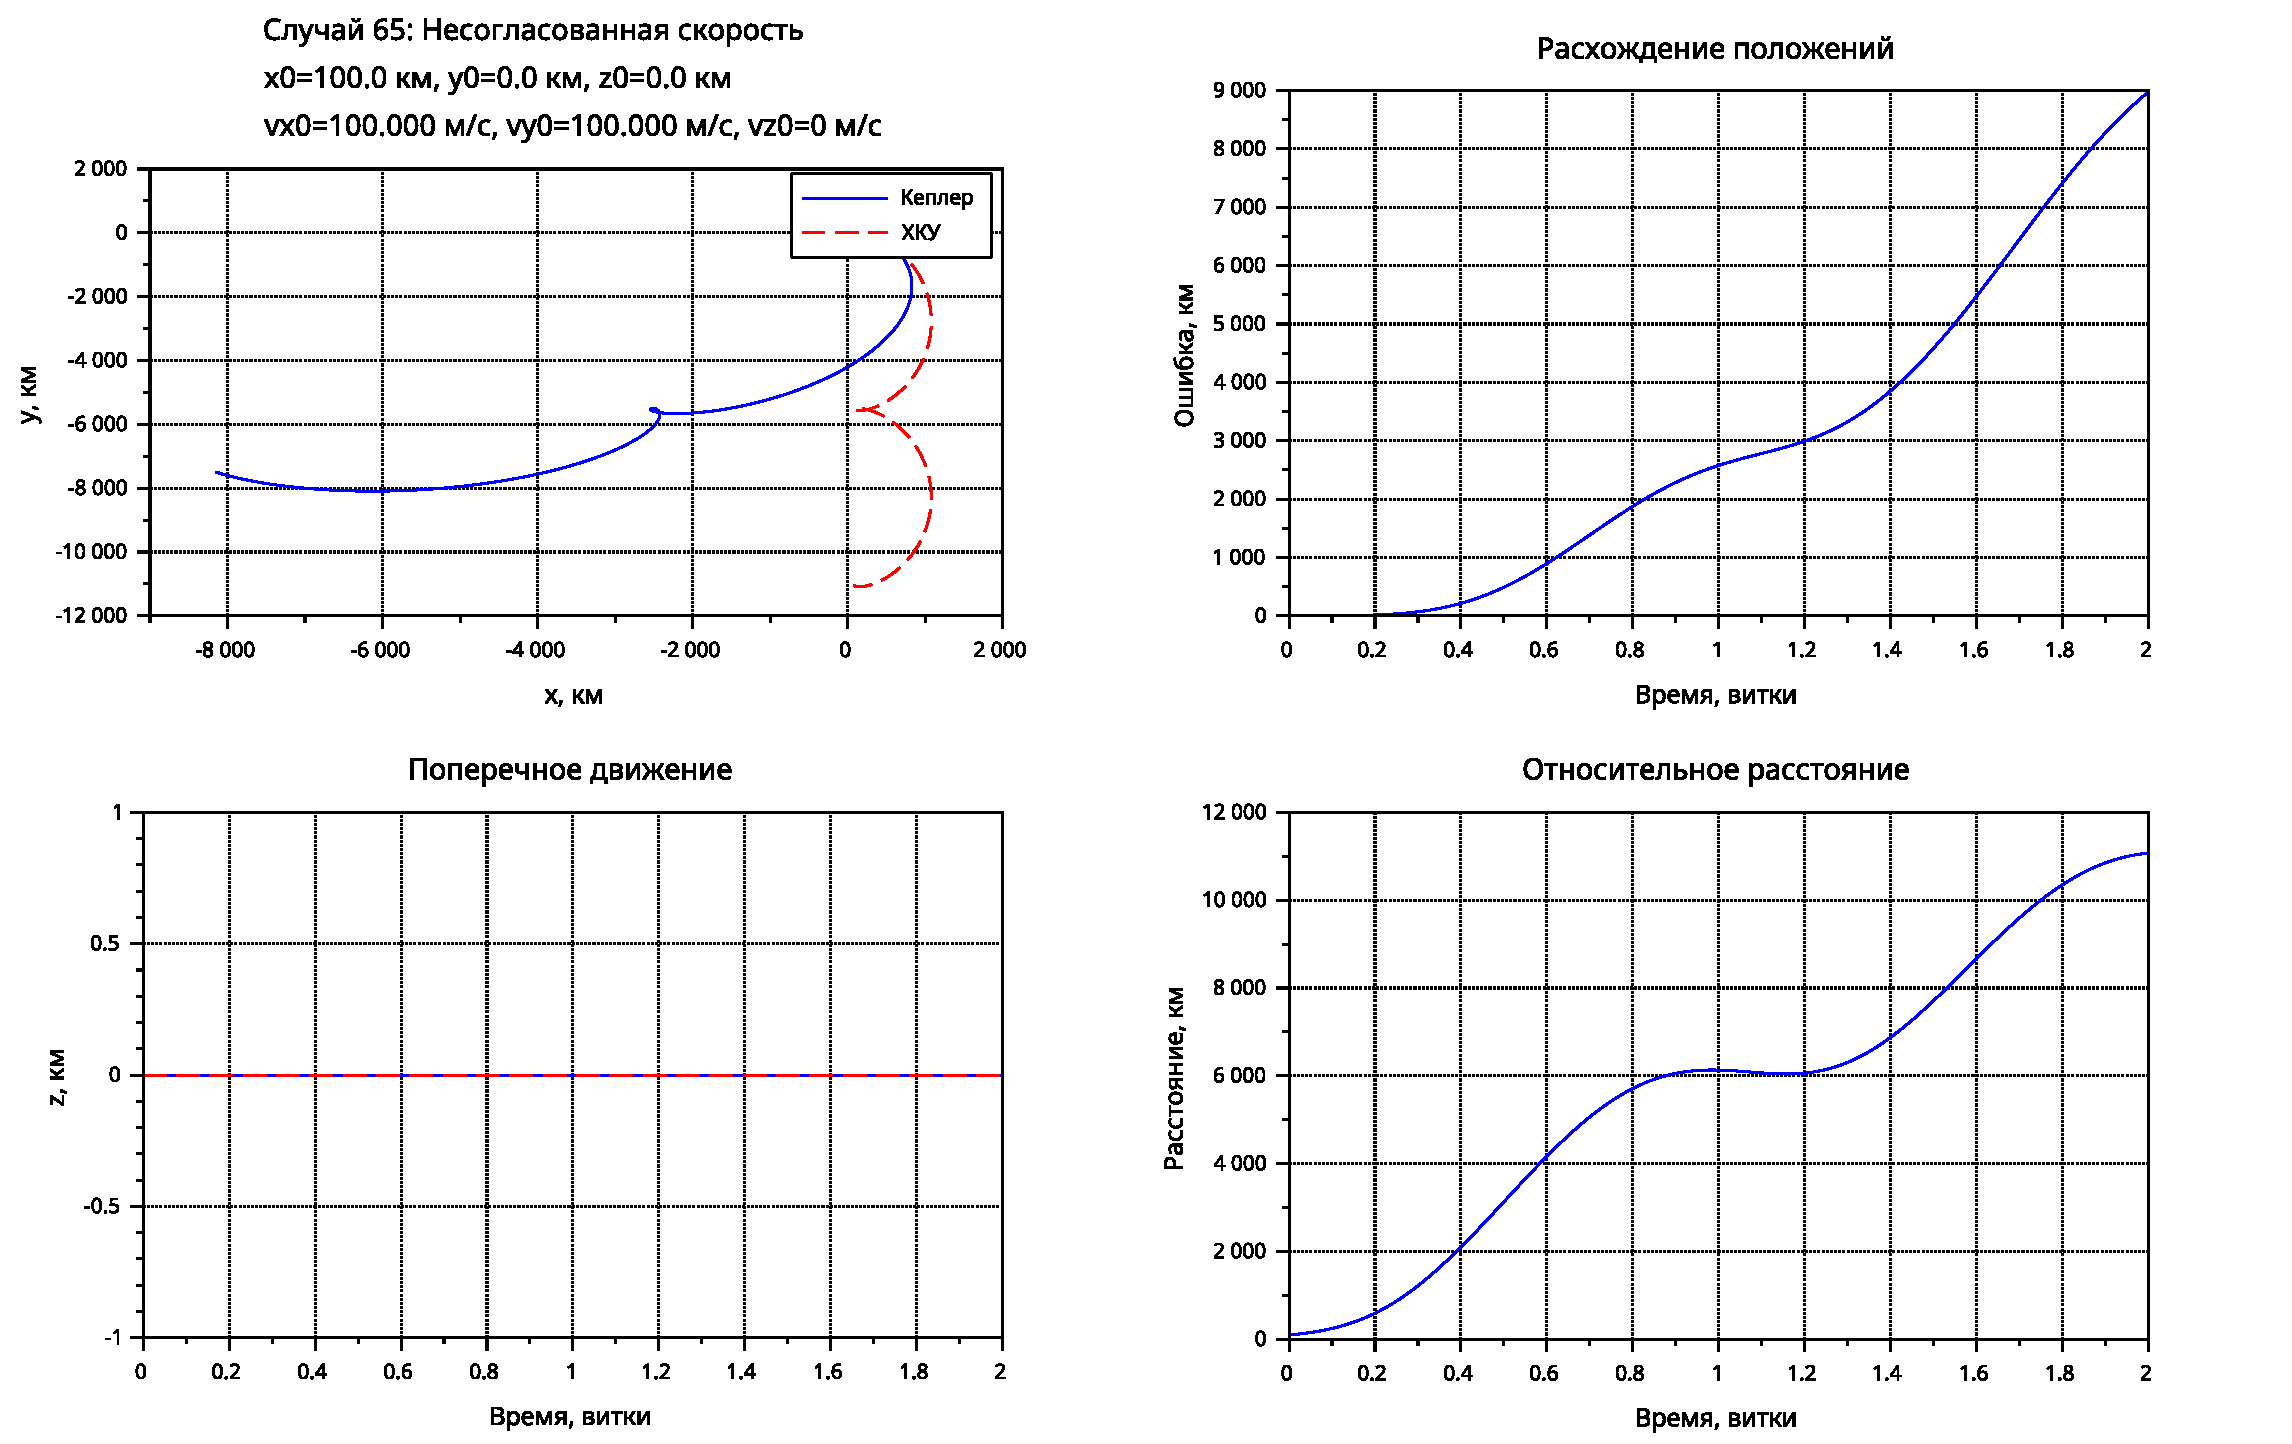
\includegraphics[width=.9\textwidth]{results/case_65.pdf}
        \caption{№65: большой разлёт, ХКУ за пределами применимости.}
    \end{figure}
    \section{Таблица результатов}
    В каждом наборе координат первой идёт согласованная скорость, затем пары несогласованных
    скоростей $(0,0)$, $(0,100)$, $(100,0)$, $(100,100)$ м/с.
    \begin{longtable}{rrrrrrrrr}
    \caption{Результаты всех начальных условий. Скорости в м/с, расстояния в км.}\\
    \toprule № & $x_0$ & $y_0$ & $z_0$ & $v_x$ & $v_y$ & $\Delta_{max}$ & $\Delta_{end}$ & $\rho_{max}/a$ \\
    \midrule
    \endfirsthead
    \toprule № & $x_0$ & $y_0$ & $z_0$ & $v_x$ & $v_y$ & $\Delta_{max}$ & $\Delta_{end}$ & $\rho_{max}/a$ \\
    \midrule
    \endhead
    1 & 0.1 & 0.0 & 0.0 & 0.000 & -0.216 & 0.00002 & 0.00001 & 0.0000 \\
    2 & 0.1 & 0.0 & 0.0 & 0.000 & 0.000 & 0.00414 & 0.00414 & 0.0011 \\
    3 & 0.1 & 0.0 & 0.0 & 0.000 & 100.000 & 928.84197 & 928.84197 & 0.5237 \\
    4 & 0.1 & 0.0 & 0.0 & 100.000 & 0.000 & 23.48452 & 23.18932 & 0.0563 \\
    5 & 0.1 & 0.0 & 0.0 & 100.000 & 100.000 & 994.68107 & 994.68107 & 0.5392 \\
    6 & 0.1 & 0.0 & 0.1 & 0.000 & -0.216 & 0.00004 & 0.00004 & 0.0000 \\
    7 & 0.1 & 0.0 & 0.1 & 0.000 & 0.000 & 0.00412 & 0.00412 & 0.0011 \\
    8 & 0.1 & 0.0 & 0.1 & 0.000 & 100.000 & 928.84198 & 928.84198 & 0.5237 \\
    9 & 0.1 & 0.0 & 0.1 & 100.000 & 0.000 & 23.48455 & 23.18931 & 0.0563 \\
    10 & 0.1 & 0.0 & 0.1 & 100.000 & 100.000 & 994.68106 & 994.68106 & 0.5392 \\
    11 & 0.1 & 0.1 & 0.0 & 0.054 & -0.216 & 0.00027 & 0.00027 & 0.0000 \\
    12 & 0.1 & 0.1 & 0.0 & 0.000 & 0.000 & 0.00403 & 0.00403 & 0.0011 \\
    13 & 0.1 & 0.1 & 0.0 & 0.000 & 100.000 & 928.79267 & 928.79267 & 0.5237 \\
    14 & 0.1 & 0.1 & 0.0 & 100.000 & 0.000 & 23.43467 & 23.13945 & 0.0563 \\
    15 & 0.1 & 0.1 & 0.0 & 100.000 & 100.000 & 994.60140 & 994.60140 & 0.5391 \\
    16 & 0.1 & 0.1 & 0.1 & 0.054 & -0.216 & 0.00025 & 0.00025 & 0.0000 \\
    17 & 0.1 & 0.1 & 0.1 & 0.000 & 0.000 & 0.00402 & 0.00402 & 0.0011 \\
    18 & 0.1 & 0.1 & 0.1 & 0.000 & 100.000 & 928.79269 & 928.79269 & 0.5237 \\
    19 & 0.1 & 0.1 & 0.1 & 100.000 & 0.000 & 23.43468 & 23.13937 & 0.0563 \\
    20 & 0.1 & 0.1 & 0.1 & 100.000 & 100.000 & 994.60134 & 994.60134 & 0.5391 \\
    21 & 0.1 & 1.0 & 0.0 & 0.539 & -0.216 & 0.00320 & 0.00320 & 0.0001 \\
    22 & 0.1 & 1.0 & 0.0 & 0.000 & 0.000 & 0.00659 & 0.00659 & 0.0009 \\
    23 & 0.1 & 1.0 & 0.0 & 0.000 & 100.000 & 928.35197 & 928.35197 & 0.5236 \\
    24 & 0.1 & 1.0 & 0.0 & 100.000 & 0.000 & 22.99067 & 22.69475 & 0.0561 \\
    25 & 0.1 & 1.0 & 0.0 & 100.000 & 100.000 & 993.89329 & 993.89329 & 0.5389 \\
    26 & 0.1 & 1.0 & 0.1 & 0.539 & -0.216 & 0.00318 & 0.00317 & 0.0001 \\
    27 & 0.1 & 1.0 & 0.1 & 0.000 & 0.000 & 0.00664 & 0.00664 & 0.0009 \\
    28 & 0.1 & 1.0 & 0.1 & 0.000 & 100.000 & 928.35199 & 928.35199 & 0.5236 \\
    29 & 0.1 & 1.0 & 0.1 & 100.000 & 0.000 & 22.99069 & 22.69477 & 0.0561 \\
    30 & 0.1 & 1.0 & 0.1 & 100.000 & 100.000 & 993.89330 & 993.89330 & 0.5389 \\
    31 & 10.0 & 0.0 & 0.0 & 0.000 & -21.560 & 0.26506 & 0.26441 & 0.0029 \\
    32 & 10.0 & 0.0 & 0.0 & 0.000 & 0.000 & 41.27933 & 41.27933 & 0.1085 \\
    33 & 10.0 & 0.0 & 0.0 & 0.000 & 100.000 & 1365.49770 & 1365.49770 & 0.6351 \\
    34 & 10.0 & 0.0 & 0.0 & 100.000 & 0.000 & 67.30896 & 60.89491 & 0.1429 \\
    35 & 10.0 & 0.0 & 0.0 & 100.000 & 100.000 & 1446.57169 & 1446.57169 & 0.6485 \\
    36 & 10.0 & 0.0 & 0.1 & 0.000 & -21.560 & 0.26841 & 0.26830 & 0.0029 \\
    37 & 10.0 & 0.0 & 0.1 & 0.000 & 0.000 & 41.27933 & 41.27933 & 0.1085 \\
    38 & 10.0 & 0.0 & 0.1 & 0.000 & 100.000 & 1365.49771 & 1365.49771 & 0.6351 \\
    39 & 10.0 & 0.0 & 0.1 & 100.000 & 0.000 & 67.30897 & 60.89493 & 0.1429 \\
    40 & 10.0 & 0.0 & 0.1 & 100.000 & 100.000 & 1446.57166 & 1446.57166 & 0.6485 \\
    41 & 10.0 & 0.1 & 0.0 & 0.054 & -21.560 & 0.26860 & 0.26838 & 0.0029 \\
    42 & 10.0 & 0.1 & 0.0 & 0.000 & 0.000 & 41.26864 & 41.26864 & 0.1085 \\
    43 & 10.0 & 0.1 & 0.0 & 0.000 & 100.000 & 1365.43803 & 1365.43803 & 0.6350 \\
    44 & 10.0 & 0.1 & 0.0 & 100.000 & 0.000 & 67.27084 & 60.85644 & 0.1429 \\
    45 & 10.0 & 0.1 & 0.0 & 100.000 & 100.000 & 1446.47917 & 1446.47917 & 0.6485 \\
    46 & 10.0 & 0.1 & 0.1 & 0.054 & -21.560 & 0.26858 & 0.26835 & 0.0029 \\
    47 & 10.0 & 0.1 & 0.1 & 0.000 & 0.000 & 41.26865 & 41.26865 & 0.1085 \\
    48 & 10.0 & 0.1 & 0.1 & 0.000 & 100.000 & 1365.43809 & 1365.43809 & 0.6350 \\
    49 & 10.0 & 0.1 & 0.1 & 100.000 & 0.000 & 67.27047 & 60.85593 & 0.1429 \\
    50 & 10.0 & 0.1 & 0.1 & 100.000 & 100.000 & 1446.47921 & 1446.47921 & 0.6485 \\
    51 & 10.0 & 1.0 & 0.0 & 0.539 & -21.560 & 0.26704 & 0.26501 & 0.0029 \\
    52 & 10.0 & 1.0 & 0.0 & 0.000 & 0.000 & 41.17368 & 41.17368 & 0.1083 \\
    53 & 10.0 & 1.0 & 0.0 & 0.000 & 100.000 & 1364.90472 & 1364.90472 & 0.6349 \\
    54 & 10.0 & 1.0 & 0.0 & 100.000 & 0.000 & 66.93104 & 60.51381 & 0.1427 \\
    55 & 10.0 & 1.0 & 0.0 & 100.000 & 100.000 & 1445.64964 & 1445.64964 & 0.6483 \\
    56 & 10.0 & 1.0 & 0.1 & 0.539 & -21.560 & 0.26701 & 0.26498 & 0.0029 \\
    57 & 10.0 & 1.0 & 0.1 & 0.000 & 0.000 & 41.17371 & 41.17371 & 0.1083 \\
    58 & 10.0 & 1.0 & 0.1 & 0.000 & 100.000 & 1364.90474 & 1364.90474 & 0.6349 \\
    59 & 10.0 & 1.0 & 0.1 & 100.000 & 0.000 & 66.93105 & 60.51381 & 0.1427 \\
    60 & 10.0 & 1.0 & 0.1 & 100.000 & 100.000 & 1445.64965 & 1445.64965 & 0.6483 \\
    61 & 100.0 & 0.0 & 0.0 & 0.000 & -215.602 & 25.98556 & 25.78865 & 0.0322 \\
    62 & 100.0 & 0.0 & 0.0 & 0.000 & 0.000 & 4142.09494 & 4142.09494 & 1.0973 \\
    63 & 100.0 & 0.0 & 0.0 & 0.000 & 100.000 & 8721.74988 & 8721.74988 & 1.5696 \\
    64 & 100.0 & 0.0 & 0.0 & 100.000 & 0.000 & 4300.59670 & 4300.59670 & 1.1067 \\
    65 & 100.0 & 0.0 & 0.0 & 100.000 & 100.000 & 8978.22903 & 8978.22903 & 1.5816 \\
    66 & 100.0 & 0.0 & 0.1 & 0.000 & -215.602 & 25.98553 & 25.78862 & 0.0322 \\
    67 & 100.0 & 0.0 & 0.1 & 0.000 & 0.000 & 4142.09496 & 4142.09496 & 1.0973 \\
    68 & 100.0 & 0.0 & 0.1 & 0.000 & 100.000 & 8721.74991 & 8721.74991 & 1.5696 \\
    69 & 100.0 & 0.0 & 0.1 & 100.000 & 0.000 & 4300.59668 & 4300.59668 & 1.1067 \\
    70 & 100.0 & 0.0 & 0.1 & 100.000 & 100.000 & 8978.22900 & 8978.22900 & 1.5816 \\
    71 & 100.0 & 0.1 & 0.0 & 0.054 & -215.602 & 25.98779 & 25.78830 & 0.0322 \\
    72 & 100.0 & 0.1 & 0.0 & 0.000 & 0.000 & 4141.99160 & 4141.99160 & 1.0973 \\
    73 & 100.0 & 0.1 & 0.0 & 0.000 & 100.000 & 8721.61004 & 8721.61004 & 1.5696 \\
    74 & 100.0 & 0.1 & 0.0 & 100.000 & 0.000 & 4300.44866 & 4300.44866 & 1.1067 \\
    75 & 100.0 & 0.1 & 0.0 & 100.000 & 100.000 & 8978.03492 & 8978.03492 & 1.5816 \\
    76 & 100.0 & 0.1 & 0.1 & 0.054 & -215.602 & 25.98777 & 25.78828 & 0.0322 \\
    77 & 100.0 & 0.1 & 0.1 & 0.000 & 0.000 & 4141.99162 & 4141.99162 & 1.0973 \\
    78 & 100.0 & 0.1 & 0.1 & 0.000 & 100.000 & 8721.61007 & 8721.61007 & 1.5696 \\
    79 & 100.0 & 0.1 & 0.1 & 100.000 & 0.000 & 4300.44867 & 4300.44867 & 1.1067 \\
    80 & 100.0 & 0.1 & 0.1 & 100.000 & 100.000 & 8978.03495 & 8978.03495 & 1.5816 \\
    81 & 100.0 & 1.0 & 0.0 & 0.539 & -215.602 & 26.00765 & 25.78550 & 0.0322 \\
    82 & 100.0 & 1.0 & 0.0 & 0.000 & 0.000 & 4141.06573 & 4141.06573 & 1.0972 \\
    83 & 100.0 & 1.0 & 0.0 & 0.000 & 100.000 & 8720.35803 & 8720.35803 & 1.5695 \\
    84 & 100.0 & 1.0 & 0.0 & 100.000 & 0.000 & 4299.12085 & 4299.12085 & 1.1065 \\
    85 & 100.0 & 1.0 & 0.0 & 100.000 & 100.000 & 8976.29295 & 8976.29295 & 1.5815 \\
    86 & 100.0 & 1.0 & 0.1 & 0.539 & -215.602 & 26.00763 & 25.78547 & 0.0322 \\
    87 & 100.0 & 1.0 & 0.1 & 0.000 & 0.000 & 4141.06575 & 4141.06575 & 1.0972 \\
    88 & 100.0 & 1.0 & 0.1 & 0.000 & 100.000 & 8720.35806 & 8720.35806 & 1.5695 \\
    89 & 100.0 & 1.0 & 0.1 & 100.000 & 0.000 & 4299.12090 & 4299.12090 & 1.1065 \\
    90 & 100.0 & 1.0 & 0.1 & 100.000 & 100.000 & 8976.29298 & 8976.29298 & 1.5815 \\
    \bottomrule
\end{longtable}

\end{document}
